\documentclass[11pt,a4paper]{article}

%% ── Packages ──────────────────────────────────────────────────────────
\usepackage[margin=2.5cm]{geometry}
\usepackage[T1]{fontenc}
\usepackage[utf8]{inputenc}
\usepackage{lmodern}
\usepackage{microtype}
\usepackage{booktabs}
\usepackage{longtable}
\usepackage{array}
\usepackage{tabularx}
\usepackage{xcolor}
\usepackage{graphicx}
\usepackage{float}
\usepackage{enumitem}
\usepackage{listings}
\usepackage{caption}
\usepackage{subcaption}
\usepackage{amsmath}
\usepackage{amssymb}
\usepackage{parskip}
\usepackage{fancyhdr}
\usepackage{titlesec}
\usepackage[hidelinks,colorlinks=true,linkcolor=NavyBlue,urlcolor=NavyBlue]{hyperref}
\usepackage{tikz}
\usetikzlibrary{shapes,shapes.geometric,arrows.meta,positioning,calc,fit,backgrounds,decorations.pathreplacing}
\usepackage{pgfplots}
\pgfplotsset{compat=1.18}
\usepackage{colortbl}

%% ── Colours ───────────────────────────────────────────────────────────
\definecolor{NavyBlue}{HTML}{1A4A8A}
\definecolor{SteelBlue}{HTML}{4472C4}
\definecolor{LightBlue}{HTML}{DAE9F8}
\definecolor{DarkGreen}{HTML}{1E7030}
\definecolor{MedGreen}{HTML}{70AD47}
\definecolor{LightGreen}{HTML}{E2EFDA}
\definecolor{DarkRed}{HTML}{C00000}
\definecolor{LightRed}{HTML}{FFE0E0}
\definecolor{Amber}{HTML}{ED7D31}
\definecolor{LightAmber}{HTML}{FFF2CC}
\definecolor{LightGray}{HTML}{F5F5F5}
\definecolor{MedGray}{HTML}{D0D0D0}
\definecolor{CodeBg}{HTML}{F8F8F8}
\definecolor{CommentGreen}{HTML}{5A8A5A}
\definecolor{StringRed}{HTML}{A31515}
\definecolor{KeywordBlue}{HTML}{0000CC}

%% ── Code listings ─────────────────────────────────────────────────────
\lstdefinestyle{python}{
  language=Python,
  basicstyle=\footnotesize\ttfamily,
  backgroundcolor=\color{CodeBg},
  keywordstyle=\color{KeywordBlue}\bfseries,
  commentstyle=\color{CommentGreen}\itshape,
  stringstyle=\color{StringRed},
  showstringspaces=false,
  breaklines=true,
  frame=single,
  framesep=4pt,
  rulecolor=\color{MedGray},
  xleftmargin=8pt,
  xrightmargin=4pt,
  numbers=left,
  numberstyle=\tiny\color{gray},
  numbersep=6pt,
  tabsize=4,
  columns=flexible,
  keepspaces=true,
  upquote=true,
  belowskip=0.5em,
  aboveskip=0.5em,
}

\lstdefinestyle{typescript}{
  language=Java,
  basicstyle=\footnotesize\ttfamily,
  backgroundcolor=\color{CodeBg},
  keywordstyle=\color{KeywordBlue}\bfseries,
  commentstyle=\color{CommentGreen}\itshape,
  stringstyle=\color{StringRed},
  showstringspaces=false,
  breaklines=true,
  frame=single,
  framesep=4pt,
  rulecolor=\color{MedGray},
  xleftmargin=8pt,
  numbers=left,
  numberstyle=\tiny\color{gray},
  numbersep=6pt,
  tabsize=2,
  columns=flexible,
  keepspaces=true,
  upquote=true,
  belowskip=0.5em,
  aboveskip=0.5em,
}

\lstdefinestyle{inline}{
  basicstyle=\small\ttfamily,
  backgroundcolor=\color{CodeBg},
  frame=none,
  breaklines=true,
}

%% ── Section styling ───────────────────────────────────────────────────
\titleformat{\section}
  {\large\bfseries\color{NavyBlue}}
  {\thesection}{0.8em}{}[\vspace{-0.3em}\rule{\textwidth}{1.5pt}]

\titleformat{\subsection}
  {\normalsize\bfseries\color{SteelBlue}}
  {\thesubsection}{0.8em}{}

\titleformat{\subsubsection}
  {\small\bfseries\color{SteelBlue}}
  {\thesubsubsection}{0.8em}{}

%% ── Header / Footer ───────────────────────────────────────────────────
\pagestyle{fancy}
\fancyhf{}
\renewcommand{\headrulewidth}{0.4pt}
\fancyhead[L]{\small\color{gray} ResearchShop --- Pipeline Internals}
\fancyhead[R]{\small\color{gray} \today}
\fancyfoot[C]{\small\color{gray}\thepage}

%% ── Callout boxes ─────────────────────────────────────────────────────
\newcommand{\warnbox}[2]{%
  \vspace{0.4em}
  \noindent\colorbox{LightRed}{\parbox{\dimexpr\linewidth-2\fboxsep}{%
    \small\color{DarkRed}\textbf{[#1]}\quad #2}}
  \vspace{0.4em}
}

\newcommand{\notebox}[1]{%
  \vspace{0.4em}
  \noindent\colorbox{LightBlue}{\parbox{\dimexpr\linewidth-2\fboxsep}{%
    \small\color{NavyBlue}\textbf{Note:}\quad #1}}
  \vspace{0.4em}
}

\newcommand{\codefile}[1]{\texttt{\small\color{gray}#1}}

%% ── Document ──────────────────────────────────────────────────────────
\begin{document}

%% ════════════════════════════════════════════════════════════════════
%% COVER PAGE
%% ════════════════════════════════════════════════════════════════════
\begin{titlepage}
  \centering
  \vspace*{3cm}
  {\huge\bfseries\color{NavyBlue} ResearchShop Pipeline}\par
  \vspace{0.5em}
  {\Large\color{SteelBlue} Technical Internals Report}\par
  \vspace{2em}
  \rule{0.6\textwidth}{1pt}\par
  \vspace{1.5em}
  {\normalsize
    A complete technical reference for the gene extraction pipeline:\\[0.4em]
    architecture, data flow, module internals, benchmark results,\\[0.4em]
    configuration flags, and known issues.
  }\par
  \vspace{2em}
  \rule{0.6\textwidth}{0.4pt}\par
  \vspace{1em}
  {\small\color{gray}Generated \today \ from source at \texttt{RS\_SOFTWAREX/}}\par
  \vfill
  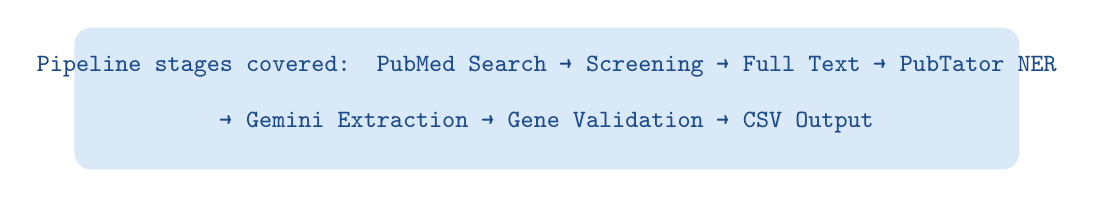
\begin{tikzpicture}
    \fill[LightBlue,rounded corners=6pt] (0,0) rectangle (12,1.8);
    \node[font=\small\ttfamily,color=NavyBlue] at (6,1.3)
      {\textbf{Pipeline stages covered:} PubMed Search → Screening → Full Text → PubTator NER};
    \node[font=\small\ttfamily,color=NavyBlue] at (6,0.6)
      {→ Gemini Extraction → Gene Validation → CSV Output};
  \end{tikzpicture}
\end{titlepage}

%% ════════════════════════════════════════════════════════════════════
%% TABLE OF CONTENTS
%% ════════════════════════════════════════════════════════════════════
\tableofcontents
\newpage

%% ════════════════════════════════════════════════════════════════════
\section{Architecture Overview}
%% ════════════════════════════════════════════════════════════════════

\subsection{System diagram}

The pipeline spans two processes: an \textbf{Electron renderer} (TypeScript, UI) and a \textbf{Python subprocess} (spawned on each run). They communicate over stdout/stdin using a newline-delimited JSON protocol.

\begin{figure}[H]
\centering
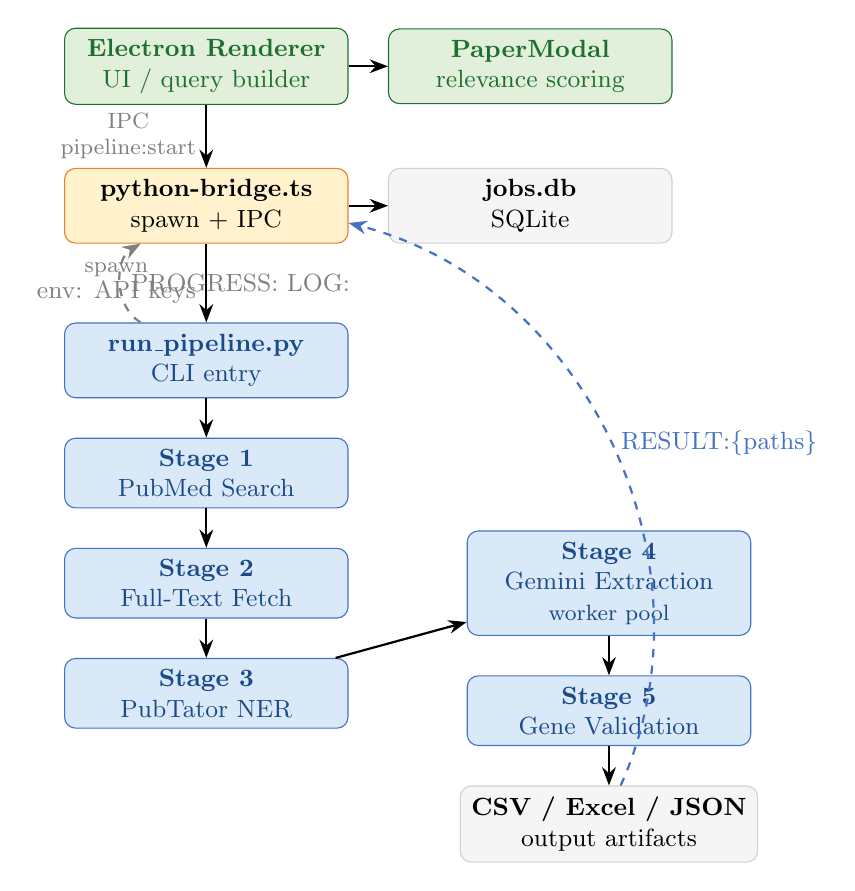
\begin{tikzpicture}[
  box/.style={rectangle,rounded corners=4pt,minimum width=3.6cm,minimum height=0.75cm,
              font=\small,align=center,inner sep=4pt},
  arrow/.style={-Stealth,thick},
  stage/.style={box,fill=LightBlue,draw=SteelBlue,text=NavyBlue},
  electron/.style={box,fill=LightGreen,draw=DarkGreen,text=DarkGreen},
  bridge/.style={box,fill=LightAmber,draw=Amber,text=black},
  io/.style={box,fill=LightGray,draw=MedGray,text=black},
  label/.style={font=\footnotesize\color{gray},align=center},
  node distance=0.5cm
]

%% Electron side
\node[electron] (ui)        {\textbf{Electron Renderer}\\UI / query builder};
\node[electron,right=0.5cm of ui] (modal)   {\textbf{PaperModal}\\relevance scoring};
\node[bridge,below=0.8cm of ui]   (bridge)  {\textbf{python-bridge.ts}\\spawn + IPC};
\node[io,right=0.5cm of bridge]   (idb)     {\textbf{jobs.db}\\SQLite};

%% Python side
\node[stage,below=1.0cm of bridge]  (entry)   {\textbf{run\_pipeline.py}\\CLI entry};
\node[stage,below=0.5cm of entry]   (s1)      {\textbf{Stage 1}\\PubMed Search};
\node[stage,below=0.5cm of s1]      (s2)      {\textbf{Stage 2}\\Full-Text Fetch};
\node[stage,below=0.5cm of s2]      (s3)      {\textbf{Stage 3}\\PubTator NER};
\node[stage,right=1.5cm of s2]      (s4)      {\textbf{Stage 4}\\Gemini Extraction\\{\footnotesize worker pool}};
\node[stage,below=0.5cm of s4]      (s5)      {\textbf{Stage 5}\\Gene Validation};
\node[io,below=0.5cm of s5]         (csv)     {\textbf{CSV / Excel / JSON}\\output artifacts};

%% Arrows
\draw[arrow] (ui) -- (modal);
\draw[arrow] (ui) -- node[label,left]{IPC\\pipeline:start} (bridge);
\draw[arrow] (bridge) -- (idb);
\draw[arrow] (bridge) -- node[label,left]{spawn\\\small env: API keys} (entry);
\draw[arrow] (entry) -- (s1);
\draw[arrow] (s1) -- (s2);
\draw[arrow] (s2) -- (s3);
\draw[arrow] (s3) -- (s4);
\draw[arrow] (s4) -- (s5);
\draw[arrow] (s5) -- (csv);

\draw[arrow,dashed,color=SteelBlue] (csv) to[bend right=50]
  node[label,right]{\small RESULT:\{paths\}} (bridge);
\draw[arrow,dashed,color=gray] (entry) to[bend left=60]
  node[label,right]{\small PROGRESS:\ LOG:} (bridge);

\end{tikzpicture}
\caption{High-level system architecture. Dashed arrows show the stdout IPC protocol flowing back to the Electron main process.}
\end{figure}

\subsection{The three trust tiers}

The design resolves a fundamental tension: PubTator has high precision but low recall; Gemini has high recall but can hallucinate. The pipeline layers them:

\begin{center}
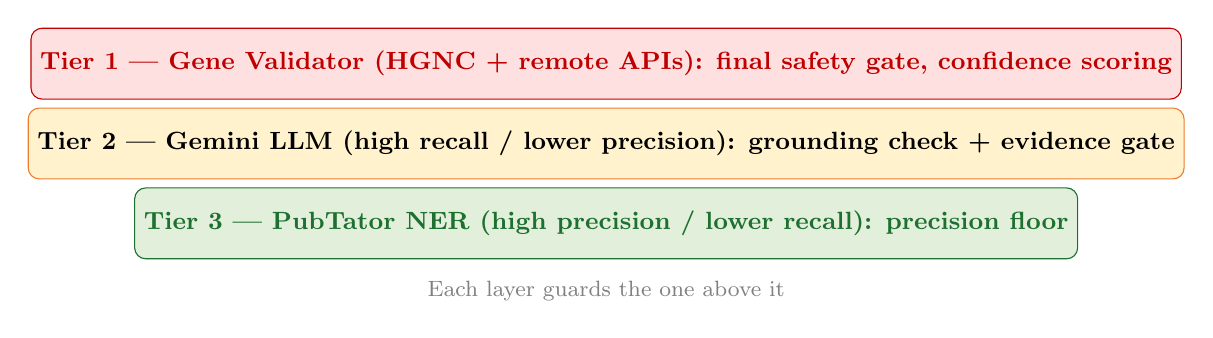
\begin{tikzpicture}[
  tier/.style={rectangle,rounded corners=4pt,minimum width=10cm,minimum height=0.9cm,
               font=\small\bfseries,align=center},
  node distance=0.1cm
]
\node[tier,fill=LightRed,draw=DarkRed,text=DarkRed]
  (t1) {\textbf{Tier 1 — Gene Validator} (HGNC + remote APIs): final safety gate, confidence scoring};
\node[tier,fill=LightAmber,draw=Amber,below=0.1cm of t1]
  (t2) {\textbf{Tier 2 — Gemini LLM} (high recall / lower precision): grounding check + evidence gate};
\node[tier,fill=LightGreen,draw=DarkGreen,text=DarkGreen,below=0.1cm of t2]
  (t3) {\textbf{Tier 3 — PubTator NER} (high precision / lower recall): precision floor};
\node[font=\footnotesize\color{gray},below=0.15cm of t3] {Each layer guards the one above it};
\end{tikzpicture}
\end{center}

\subsection{The two process models}

\begin{center}
\begin{tabular}{lll}
\toprule
\textbf{Mode} & \textbf{Config} & \textbf{Behaviour} \\
\midrule
Sequential (default) & \texttt{PARALLEL\_ANALYSIS=false} & One paper at a time. Safe for free-tier Gemini (15 RPM). \\
Parallel & \texttt{PARALLEL\_ANALYSIS=true} & Multiple in-flight. For paid keys. Pool size: 2--4. \\
\bottomrule
\end{tabular}
\end{center}

%% ════════════════════════════════════════════════════════════════════
\section{IPC Protocol}
%% ════════════════════════════════════════════════════════════════════

Python writes newline-delimited JSON to stdout. The Electron bridge parses it in a line buffer.

\begin{center}
\begin{tabular}{lll}
\toprule
\textbf{Prefix} & \textbf{Required fields} & \textbf{Optional / notes} \\
\midrule
\texttt{PROGRESS:} & \texttt{stage}, \texttt{percent} & \texttt{stats.gemini\_api\_calls}, \texttt{stats.genes\_extracted} \\
\texttt{LOG:}      & \texttt{level}, \texttt{msg}     & \texttt{detail} (nullable) \\
\texttt{RESULT:}   & \textit{none enforced}            & \texttt{local\_path}, \texttt{metadata\_path}, \texttt{excel\_path}, \texttt{json\_path}, \texttt{error} \\
\bottomrule
\end{tabular}
\end{center}

\warnbox{Bug \#1.8}{The \texttt{isResultPayload} type guard (\codefile{python-bridge.ts:26}) accepts any non-null object --- including \texttt{\{\}}. A Python bug that emits \texttt{RESULT:\{\}} marks the job \textit{completed} with null artifact paths.}

\begin{lstlisting}[style=python,caption={\codefile{run\_pipeline.py:46--52} --- Emit protocol with mandatory flush}]
def progress_callback(stage, pct, stats):
    msg = json.dumps({"stage": stage, "percent": pct, "stats": stats})
    print(f"PROGRESS:{msg}", flush=True)   # flush=True is mandatory

def log_callback(level, msg, detail=None):
    payload = json.dumps({"level": level, "msg": msg, "detail": detail})
    print(f"LOG:{payload}", flush=True)
\end{lstlisting}

Secrets are passed only via environment variables (\texttt{GEMINI\_API\_KEY}, \texttt{ENTREZ\_EMAIL}). CLI args are visible in \texttt{ps aux} output and are never used for secrets.

%% ════════════════════════════════════════════════════════════════════
\section{Pipeline Stages}
%% ════════════════════════════════════════════════════════════════════

\subsection{Stage 1 --- PubMed Search \& Citation Ranking}
\codefile{python/modules/pubmed\_data\_collector.py} (457 lines)

Queries NCBI Entrez, applies the OA filter (\texttt{"loattrfull text[sb]"}), and ranks results by citation count.

\textbf{Citation ranking chain:} iCite (NIH, batch) $\to$ Semantic Scholar (fallback, per-PMID with 200\,ms sleep). If both fail, results are unranked.

\textbf{Overfetch factor:} \texttt{ANALYSIS\_OVERFETCH\_FACTOR=4}. If the user requests top-10 papers, 40 candidates are analysed. Compensates for paywalled papers and low-extraction failures.

\warnbox{Suspect \#2.4}{Semantic Scholar fallback is per-PMID with 200\,ms sleep. For 1000 unresolved PMIDs: $>$3 minutes of pure waiting. Batch API exists but is not used.}

\subsection{Stage 2 --- Gene Relevance Scoring (UI-side)}
\codefile{src/renderer/utils/geneRelevanceScorer.ts}

Since 2026-03-02, relevance scoring moved from the Python pipeline to the Electron renderer. Users see tier badges (\textbf{high} $\geq$10, \textbf{medium} $\geq$5, \textbf{low} 1--4, \textbf{none} $\leq$0) and can override the filter. The pipeline receives only the user's final PMID selection --- no silent post-submission filtering.

The Python \texttt{abstract\_screener.py} is retained for benchmarking and writes forensic \texttt{ScreeningDecision} records to the debug artifact, but no longer gates papers.

\subsection{Stage 3 --- Full-Text Fetch}
\codefile{python/modules/full\_text\_fetcher.py} (1036 lines)

\textbf{Strategy chain:} PMC JATS XML $\to$ Europe PMC $\to$ abstract-only.

Section keys produced: \texttt{abstract}, \texttt{introduction}, \texttt{methods}, \texttt{results}, \texttt{discussion}, \texttt{conclusion}, \texttt{supplementary}, \texttt{\_preamble}.

Figures are downloaded (max 3 per paper, max 5\,MB each) and passed as image bytes to the Gemini multimodal stage. Supplementary CSV/Excel/ZIP files are parsed separately.

\textbf{Greek letter transliteration (W1 fix):} $\alpha\to$alpha, $\beta\to$beta etc. prevents gene variant strings like $\beta$-globin being corrupted.

\subsection{Stage 4 --- PubTator NER}
\codefile{python/modules/pubtator\_tool.py} (620 lines)

Submits PMIDs to the NCBI PubTator3 BioC API in batches of 10. Returns high-precision gene symbols as the \textit{precision floor} for the hybrid architecture. Parse errors on individual papers in a batch are silently skipped (W10 --- accepted known limitation).

\subsection{Stage 5 --- Gemini Extraction}
\codefile{python/modules/gemini\_extractor.py} (2230 lines)

The most complex module. See Section~\ref{sec:gemini} for full detail.

\subsection{Stage 6 --- Gene Validation}
\codefile{python/modules/gene\_validator.py} (1122 lines)

\textbf{Source chain:} Local HGNC JSON (44,933 genes) $\to$ HGNC REST API $\to$ MyGene.info $\to$ fuzzy match.

Returns \texttt{validation\_confidence} (0.0--1.0) and \texttt{validation\_source}. The confidence threshold \texttt{FINAL\_VALIDATION\_MIN\_CONFIDENCE=0.7} is a medical accuracy decision --- do not lower without benchmark evaluation.

Citation validation uses dense sequence matching (\texttt{difflib.SequenceMatcher}) with a 0.85 ratio threshold and gene context window of $\pm$1500 characters.

\subsection{Stage 7 --- Orchestration \& CSV Output}
\codefile{python/modules/pipeline\_orchestrator.py} (1686 lines)

Manages the worker pool, aggregates results, computes confidence tiers, deduplicates, and writes four output artifacts: primary CSV, metadata CSV, Excel workbook (two sheets), JSON.

%% ════════════════════════════════════════════════════════════════════
\section{Gemini Extraction Deep Dive}
\label{sec:gemini}
%% ════════════════════════════════════════════════════════════════════

\subsection{Class lifecycle and mutable state}

\texttt{GeneInfoPipeline} is instantiated \textit{once per paper} inside the worker process. State never leaks across papers.

\begin{center}
\begin{tabular}{lll}
\toprule
\textbf{Attribute} & \textbf{Type} & \textbf{Lifecycle} \\
\midrule
\texttt{paper\_text} & \texttt{str} & Set in \texttt{\_\_init\_\_}; may be truncated by context validation \\
\texttt{original\_paper\_text} & \texttt{str} & Set in \texttt{\_\_init\_\_}; immutable backup \\
\texttt{associations} & \texttt{List[Dict]} & Reset in step 0; mutated by each discovery stage \\
\texttt{candidate\_meta} & \texttt{Dict[Tuple, Dict]} & Reset in step 0; accumulates provenance for all candidates \\
\texttt{dropped\_candidates} & \texttt{List[Dict]} & Reset in step 0; audit trail for dropped genes \\
\texttt{strict\_gate\_drops} & \texttt{List[Dict]} & Reset in step 0; confidence gate drops \\
\texttt{\_paper\_api\_calls} & \texttt{int} & Incremented on each LLM call; returned to orchestrator \\
\bottomrule
\end{tabular}
\end{center}

\subsection{The \texttt{run\_pipeline()} orchestrator}

After the 2026-04-07 readability refactor, the main method is a 25-line orchestrator delegating to five named sub-stages:

\begin{lstlisting}[style=python,caption={\codefile{gemini\_extractor.py:1318--1356} --- post-refactor orchestrator}]
def run_pipeline(self, column_descriptions):
    # Step 0: Validate and prepare paper text for context windows
    context_validation = self._validate_and_prepare_paper_text()
    if context_validation["failed"]:
        return pd.DataFrame()

    # Steps 0.5-1.5: Candidate discovery
    self._run_candidate_discovery()

    # Step 1.6: Grounding check
    self._run_grounding_check()

    # Step 2: Gene validation + normalization
    self._run_validation_and_normalize()

    # Step 3: Detail extraction
    extracted_info = self._run_detail_extraction(column_descriptions)
    if not extracted_info:
        return pd.DataFrame()

    # Step 4: Post-validation (metadata, strict gate, citation, evidence gate)
    df = pd.DataFrame(extracted_info)
    if "variant_name" in df.columns:
        df["variant_name"] = df["variant_name"].apply(
            self._normalize_variant_value)
    return self._run_post_validation(df, column_descriptions,
                                     context_validation)
\end{lstlisting}

\subsection{The five sub-stages}

\begin{description}[leftmargin=2em]
\item[\texttt{\_run\_candidate\_discovery()}]
  Steps 0.5--1.5. Resets all mutable state, then runs: abstract pass (LLM), full-text pass $\times 2$ (temperature 0.0 then 0.4), HGNC deterministic lexicon, figure multimodal analysis, PubTator merge. Each source contributes to \texttt{candidate\_meta} with a source label (\texttt{llm\_text}, \texttt{llm\_abstract}, \texttt{pubtator}, \texttt{deterministic\_lexicon}, \texttt{llm\_figure}).

\item[\texttt{\_run\_grounding\_check()}]
  Step 1.6. The primary hallucination filter. Each candidate is searched for in the paper text using its canonical symbol, HGNC aliases, and raw LLM labels (e.g. ``BNP'' for NPPB). Figure-only genes use a lighter caption-text check. Ungrounded candidates are dropped and marked \texttt{rejected\_ungrounded}.

\item[\texttt{\_run\_validation\_and\_normalize()}]
  Step 2. Calls \texttt{\_apply\_gene\_validation\_heuristics()} (HGNC chain), then ensures one gene-level row (variant = ``'') per gene. If strict gate is off and all associations are filtered, falls back to pre-validation list.

\item[\texttt{\_run\_detail\_extraction(column\_descriptions)}]
  Step 3. All validated candidates go into ONE Gemini call with the user's column schema. Returns merged, backfilled rows, or fallback rows if the LLM produced nothing.

\item[\texttt{\_run\_post\_validation(df, ...)}]
  Step 4. Adds metadata, applies strict validation gate (drops $< 0.7$ confidence), citation validation (adds \texttt{*\_citation\_valid} booleans), evidence gate (per-source evidence thresholds), and context window metadata.
\end{description}

\subsection{The four LLM extraction methods}

\begin{center}
\begin{tabular}{llll}
\toprule
\textbf{Method} & \textbf{Input} & \textbf{Max retries} & \textbf{Backoff} \\
\midrule
\texttt{extract\_gene\_names\_from\_abstract} & Abstract only & 2 & 3\,s flat \\
\texttt{extract\_gene\_names} (×2) & Full text & 3 & 5s $\times 2$ exp \\
\texttt{extract\_gene\_names\_from\_figures} & Image + caption & 3/figure & Retry-after header \\
\texttt{extract\_gene\_info} (Stage 3) & Full text + all genes & 3 & 5s $\times 2$ exp \\
\bottomrule
\end{tabular}
\end{center}

All calls use \texttt{thinking\_budget=0} (C20 fix --- preview models hang $>$600\,s without this).

\subsection{Confidence tiers}

\begin{figure}[H]
\centering
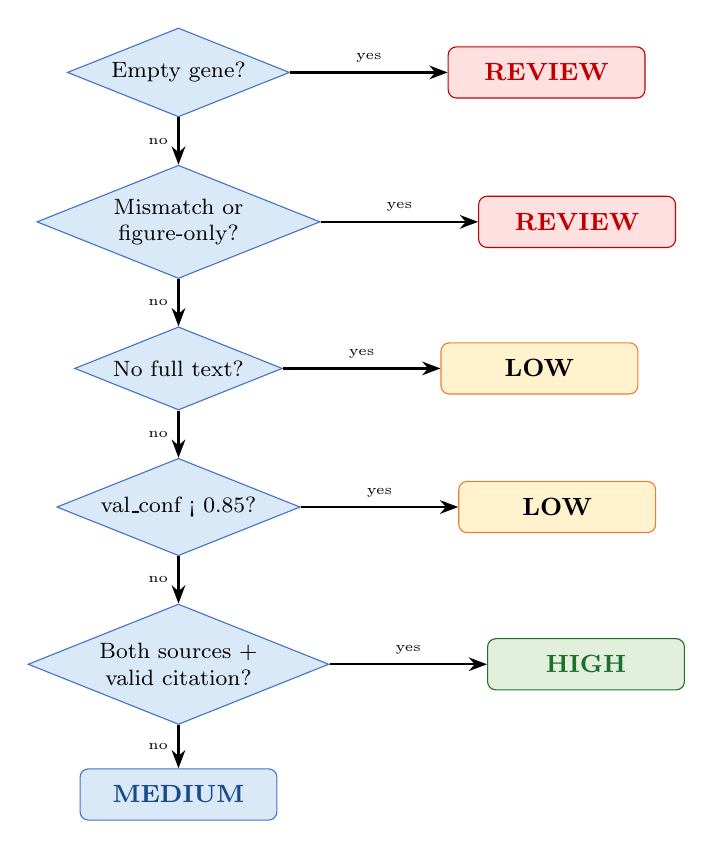
\begin{tikzpicture}[
  decision/.style={diamond,draw=SteelBlue,fill=LightBlue,aspect=2.5,
                   font=\footnotesize,align=center,inner sep=2pt},
  result/.style={rectangle,rounded corners=3pt,minimum width=2.5cm,
                 minimum height=0.65cm,font=\small\bfseries,align=center},
  arrow/.style={-Stealth,thick},
  node distance=0.6cm
]
\node[decision] (e1)  {Empty gene?};
\node[decision,below=0.6cm of e1] (e2)  {Mismatch or\\ figure-only?};
\node[decision,below=0.6cm of e2] (e3)  {No full text?};
\node[decision,below=0.6cm of e3] (e4)  {val\_conf < 0.85?};
\node[decision,below=0.6cm of e4] (e5)  {Both sources +\\ valid citation?};

\node[result,right=2cm of e1,fill=LightRed,draw=DarkRed,text=DarkRed]   (r1) {REVIEW};
\node[result,right=2cm of e2,fill=LightRed,draw=DarkRed,text=DarkRed]   (r2) {REVIEW};
\node[result,right=2cm of e3,fill=LightAmber,draw=Amber]                (r3) {LOW};
\node[result,right=2cm of e4,fill=LightAmber,draw=Amber]                (r4) {LOW};
\node[result,right=2cm of e5,fill=LightGreen,draw=DarkGreen,text=DarkGreen] (r5) {HIGH};
\node[result,below=0.55cm of e5,fill=LightBlue,draw=SteelBlue,text=NavyBlue] (r6) {MEDIUM};

\draw[arrow] (e1) -- node[above,font=\tiny]{yes} (r1);
\draw[arrow] (e1) -- node[left,font=\tiny]{no}  (e2);
\draw[arrow] (e2) -- node[above,font=\tiny]{yes} (r2);
\draw[arrow] (e2) -- node[left,font=\tiny]{no}  (e3);
\draw[arrow] (e3) -- node[above,font=\tiny]{yes} (r3);
\draw[arrow] (e3) -- node[left,font=\tiny]{no}  (e4);
\draw[arrow] (e4) -- node[above,font=\tiny]{yes} (r4);
\draw[arrow] (e4) -- node[left,font=\tiny]{no}  (e5);
\draw[arrow] (e5) -- node[above,font=\tiny]{yes} (r5);
\draw[arrow] (e5) -- node[left,font=\tiny]{no}  (r6);
\end{tikzpicture}
\caption{Confidence tier decision tree (\codefile{pipeline\_orchestrator.py:27--101}).}
\end{figure}

\warnbox{Suspect \#2.1}{HIGH is unreachable when \texttt{val\_conf} $<$ 0.85 even with dual-source corroboration. A gene confirmed by both PubTator and Gemini but with a borderline 0.80 HGNC confidence lands in LOW rather than MEDIUM.}

%% ════════════════════════════════════════════════════════════════════
\section{Benchmark Results}
%% ════════════════════════════════════════════════════════════════════

Evaluated on 12 papers across five study types, three runs each (36 total runs). Open-access full-text papers only.

\begin{figure}[H]
\centering
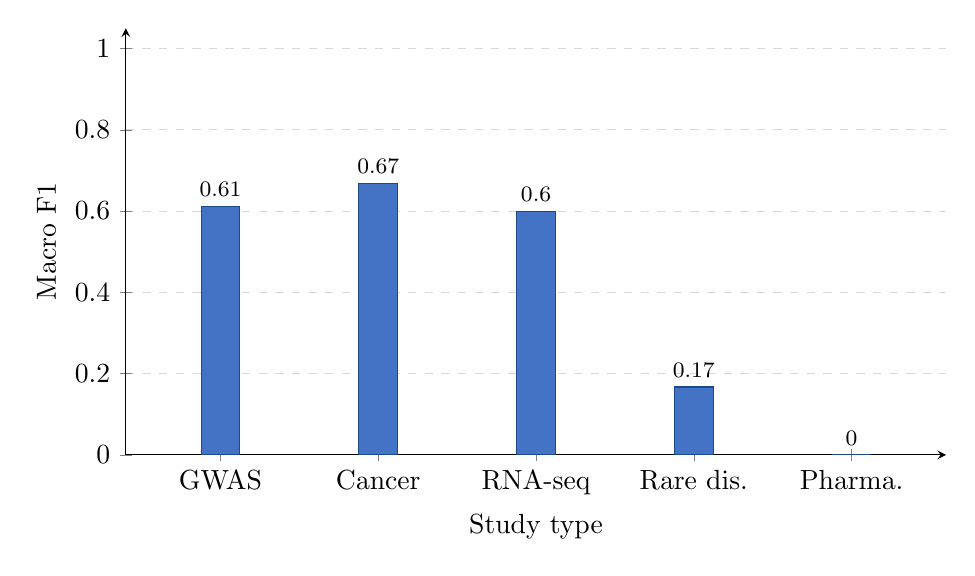
\begin{tikzpicture}
\begin{axis}[
  ybar,
  bar width=14pt,
  width=12cm, height=7cm,
  xlabel={Study type},
  ylabel={Macro F1},
  ymin=0, ymax=1.05,
  ytick={0,0.2,0.4,0.6,0.8,1.0},
  xtick=data,
  symbolic x coords={GWAS, Cancer, RNA-seq, Rare disease, Pharma.},
  xticklabels={GWAS, Cancer, RNA-seq, Rare dis., Pharma.},
  xtick align=inside,
  nodes near coords,
  nodes near coords align={vertical},
  every node near coord/.style={font=\footnotesize},
  axis lines=left,
  enlarge x limits=0.15,
  ymajorgrids=true, grid style={dashed,gray!30},
  legend style={at={(0.98,0.98)},anchor=north east,font=\small},
]
\addplot[fill=SteelBlue,draw=NavyBlue] coordinates {
  (GWAS,0.611)
  (Cancer,0.668)
  (RNA-seq,0.600)
  (Rare disease,0.167)
  (Pharma.,0.000)
};
\end{axis}
\end{tikzpicture}
\caption{Macro F1 by study type. Rare disease is low because one of the two papers (PMID 21076407) is paywalled, returning 0 genes. Pharmacogenomics F1=0 reflects that guidelines embed gene-drug associations in dosing tables, not primary research findings --- a design limitation, not a bug.}
\end{figure}

\begin{center}
\begin{tabular}{lrrrrl}
\toprule
\textbf{PMID} & \textbf{Type} & \textbf{P} & \textbf{R} & \textbf{F1} & \textbf{Notes} \\
\midrule
17463248 & GWAS              & 1.000 & 1.000 & 1.000 & T2D --- perfect extraction \\
21926974 & GWAS              & 1.000 & 0.714 & 0.833 & Schizophrenia \\
17554300 & GWAS              & 0.000 & 0.000 & 0.000 & Crohn's --- OA text issue \\
21720365 & Cancer genomics   & 0.875 & 1.000 & 0.933 & TCGA ovarian \\
23000897 & Cancer genomics   & 0.667 & 0.667 & 0.667 & TCGA breast \\
24132290 & Cancer genomics   & 0.254 & 1.000 & 0.405 & Pan-cancer; 59 genes vs 15 gold \\
20129251 & RNA-seq           & 1.000 & 1.000 & 1.000 & GBM --- figure analysis critical \\
32416070 & RNA-seq           & 1.000 & 0.111 & 0.200 & Only 1/9 gold genes extracted \\
19915526 & Rare disease      & 0.200 & 1.000 & 0.333 & Miller syndrome \\
21076407 & Rare disease      & 0.000 & 0.000 & 0.000 & Paywalled --- abstract only \\
19228618 & Pharmacogenomics  & 0.000 & 0.000 & 0.000 & Guideline document \\
22205192 & Pharmacogenomics  & 0.000 & 0.000 & 0.000 & Guideline document \\
\bottomrule
\end{tabular}
\end{center}

\textbf{Repeatability:} Jaccard similarity = 1.0 on all 12 papers across 3 runs. The gene set is perfectly reproducible run-to-run (deterministic candidate seeding).

\textbf{Figure analysis:} Controlled 36-run experiment. PMID 20129251 (GBM): F1-on = 1.000, F1-off = 0.167 ($\Delta$F1 = +0.833). Figures are the primary communication medium in comprehensive genomics papers; the LLM uses them as editorial anchors that improve precision.

%% ════════════════════════════════════════════════════════════════════
\section{Configuration Flags}
%% ════════════════════════════════════════════════════════════════════

All flags live in \codefile{python/modules/config.py}. All boolean flags accept \texttt{"true"/"false"} env vars.

\begin{longtable}{llp{4.5cm}l}
\toprule
\textbf{Flag} & \textbf{Default} & \textbf{Purpose} & \textbf{Stage} \\
\midrule
\endfirsthead
\multicolumn{4}{c}{{\tablename\ \thetable{} --- continued}} \\
\toprule
\textbf{Flag} & \textbf{Default} & \textbf{Purpose} & \textbf{Stage} \\
\midrule
\endhead
\midrule
\multicolumn{4}{r}{{Continued on next page}} \\
\endfoot
\bottomrule
\endlastfoot

\texttt{ENABLE\_OA\_FILTER}          & True  & Restrict to open-access papers               & 1 \\
\texttt{ENABLE\_PUBTATOR\_EXTRACTION}& True  & Run NER precision floor                       & 4 \\
\texttt{ENABLE\_FIGURE\_ANALYSIS}    & True  & Multimodal figure extraction                  & 5 \\
\texttt{FIGURE\_MAX\_IMAGES\_PER\_PAPER} & 3 & Cap on figures per paper                     & 5 \\
\texttt{ENABLE\_ABSTRACT\_GENE\_DISCOVERY} & True & Independent abstract-level LLM pass      & 5 \\
\texttt{ENABLE\_GROUNDING\_CHECK}    & True  & Drop genes not found in text                  & 5 \\
\texttt{ENABLE\_DETERMINISTIC\_CANDIDATES} & True & HGNC symbol regex extraction            & 5 \\
\texttt{DETERMINISTIC\_MAX\_CANDIDATES} & 120 & Cap on deterministic candidates              & 5 \\
\texttt{ENABLE\_BIOMARKER\_NORMALIZATION} & True & Resolve BNP$\to$NPPB etc.                 & 5 \\
\texttt{ENABLE\_STRICT\_VALIDATION\_GATE} & True & Drop rows below confidence threshold     & 5 \\
\texttt{FINAL\_VALIDATION\_MIN\_CONFIDENCE} & 0.7 & \textbf{Medical accuracy threshold}      & 5 \\
\texttt{ENABLE\_EVIDENCE\_BACKFILL}  & True  & Auto-fill empty Key Finding fields            & 5 \\
\texttt{ENABLE\_STRICT\_EVIDENCE\_GATE} & True & Drop rows with insufficient evidence       & 5 \\
\texttt{EVIDENCE\_MIN\_NONEMPTY\_CELLS\_LLM\_TEXT} & 0 & LLM rows trusted without backfill   & 5 \\
\texttt{EVIDENCE\_MIN\_NONEMPTY\_CELLS\_DETERMINISTIC} & 1 & Deterministic rows need corroboration & 5 \\
\texttt{ENABLE\_CITATION\_VALIDATION} & True & Validate citations exist in paper text       & 6 \\
\texttt{CITATION\_MIN\_CONFIDENCE}   & 0.7   & Citation validation threshold                 & 6 \\
\texttt{AI\_PER\_PAPER\_TIMEOUT\_SECONDS} & 600 & Worker timeout (10 min)                  & 7 \\
\texttt{AI\_WORKER\_POOL\_SIZE}      & 2     & Pool size, hard cap 4                         & 7 \\
\texttt{PARALLEL\_ANALYSIS}          & False & In-flight parallel mode                       & 7 \\
\texttt{ANALYSIS\_OVERFETCH\_FACTOR} & 4     & Fetch $4\times$ requested top-N               & 7 \\
\texttt{CONTEXT\_SAFETY\_MARGIN}     & 0.8   & Use 80\% of model context limit               & 5 \\
\texttt{GEMINI\_FLASH\_CONTEXT\_LIMIT} & 1M  & Flash model token limit                       & 5 \\
\end{longtable}

\notebox{\texttt{FINAL\_VALIDATION\_MIN\_CONFIDENCE=0.7} is a medical accuracy decision. Lowering it increases false gene associations in the output. Do not change without full benchmark evaluation.}

%% ════════════════════════════════════════════════════════════════════
\section{Known Issues \& Bugs}
%% ════════════════════════════════════════════════════════════════════

\subsection{Critical findings}

\begin{longtable}{p{0.22\textwidth}p{0.4\textwidth}p{0.28\textwidth}}
\toprule
\textbf{Location} & \textbf{Issue} & \textbf{Suggested fix} \\
\midrule
\endfirsthead
\multicolumn{3}{c}{{\tablename\ \thetable{} --- continued}} \\
\toprule \textbf{Location} & \textbf{Issue} & \textbf{Suggested fix} \\
\midrule
\endhead
\bottomrule
\endlastfoot

\rowcolor{LightRed}
\texttt{orchestrator.py:\linebreak 1085--1092} &
  Worker \texttt{.get(timeout=0)} bare \texttt{except} swallows all error types.
  Segfaults, OOM kills, assertion errors all appear as generic \texttt{"error": str(e)}.
  No traceback preserved. &
  Log \texttt{traceback.format\_exc()} and exception type before wrapping. \\

\rowcolor{LightRed}
\texttt{orchestrator.py:\linebreak 1169--1176} &
  Pool restart resets \texttt{submitted\_at} to \texttt{time.time()}. A paper that hangs twice runs
  for up to $2 \times 600\,\text{s} = 20\,\text{min}$ total before the second timeout fires. &
  Track \texttt{original\_submitted\_at} that never resets; cap at 1 restart. \\

\rowcolor{LightRed}
\texttt{orchestrator.py:\linebreak 1563--1565} &
  \texttt{\_agg\_variants} silently returns \texttt{""} for empty-variant series. Gene-level rows lose
  the ``variant\,=\,{}'' signal post-dedup, potentially shifting confidence tier. &
  Emit \texttt{"(gene-level)"} sentinel or track gene-level evidence separately. \\

\rowcolor{LightRed}
\texttt{orchestrator.py:\linebreak 1573--1574} &
  Entire dedup step wrapped in swallow-all \texttt{except}. Duplicates silently appear in output. &
  Validate dtypes before groupby; emit LOG:error on skip. \\

\rowcolor{LightRed}
\texttt{gene\_validator.py:\linebreak 704} &
  Citation dense-match threshold 0.85 is hardcoded. Paraphrased citations
  (synonyms, passive voice) never reach this ratio, causing valid rows to land in REVIEW. &
  Add \texttt{CITATION\_MATCH\_RATIO\_THRESHOLD} to config.py. \\

\rowcolor{LightRed}
\texttt{python-bridge.ts:\linebreak 25--27} &
  \texttt{isResultPayload} accepts any non-null object. \texttt{RESULT:\{\}} marks job \textit{completed} with all artifact paths null. &
  Require at least one of \texttt{local\_path | error} to be a string. \\

\rowcolor{LightRed}
\texttt{gemini\_extractor.py:\linebreak 1455--1479} &
  Grounding check bypass: genes with \texttt{sources = \{llm\_figure, deterministic\_lexicon\}}
  skip the figure-caption check and may pass on weak lexical evidence. &
  Apply figure-caption check as mandatory AND-gate for any gene with \texttt{llm\_figure} in sources. \\

\end{longtable}

\subsection{Suspect / Fragile findings}

\begin{longtable}{p{0.22\textwidth}p{0.55\textwidth}p{0.13\textwidth}}
\toprule
\textbf{Location} & \textbf{Issue} & \textbf{Severity} \\
\midrule
\endfirsthead
\multicolumn{3}{c}{{\tablename\ \thetable{} --- continued}} \\
\toprule \textbf{Location} & \textbf{Issue} & \textbf{Severity} \\
\midrule
\endhead
\bottomrule
\endlastfoot

\rowcolor{LightAmber}
\texttt{orchestrator.py:\linebreak 79--101} &
  HIGH tier unreachable when \texttt{val\_conf} $<$ 0.85, even with dual-source corroboration. &
  Suspect \\

\rowcolor{LightAmber}
\texttt{gene\_validator.py:\linebreak 216--250} &
  HGNC API fallback has no circuit breaker. 2000 genes $\times$ 8\,s timeout $= 4.5$ hours on outage. &
  Suspect \\

\rowcolor{LightAmber}
\texttt{full\_text\_fetcher.py:\linebreak 354--413} &
  Multi-panel figures (1A, 1B, 1C) sharing a URL are deduped to one entry. &
  Fragile \\

\rowcolor{LightAmber}
\texttt{pubmed\_data\_\linebreak collector.py} &
  Semantic Scholar per-PMID fallback: 1000 unresolved PMIDs $= 3+$ minutes. &
  Suspect \\

\rowcolor{LightAmber}
\texttt{python-bridge.ts:\linebreak 234--239} &
  RESULT vs.\ cancel micro-race window (microseconds; theoretical in single-threaded Node.js). &
  Fragile \\

\rowcolor{LightGray}
\texttt{orchestrator.py:\linebreak 409--517} &
  \texttt{\_finalize\_paper\_result} silently omits \texttt{Gene Source} / \texttt{NCBI Gene ID} columns when PubTator is disabled. &
  Fragile \\

\rowcolor{LightGray}
\texttt{orchestrator.py:\linebreak 217--290} &
  \texttt{\_write\_split\_output} silently drops user columns if renamed upstream. Schema mismatch between primary and metadata CSVs. &
  Fragile \\

\end{longtable}

\subsection{Hardcoded constants to move to config}

\begin{center}
\begin{tabular}{lll}
\toprule
\textbf{File:line} & \textbf{Value} & \textbf{Proposed flag} \\
\midrule
\texttt{gene\_validator.py:704} & 0.85 ratio & \texttt{CITATION\_MATCH\_RATIO\_THRESHOLD} \\
\texttt{gene\_validator.py:690} & 0.6 word overlap & \texttt{CITATION\_WORD\_OVERLAP\_THRESHOLD} \\
\texttt{gemini\_extractor.py} & 240 char snippet & already \texttt{EVIDENCE\_SNIPPET\_MAX\_CHARS} $\checkmark$ \\
\texttt{gemini\_extractor.py} & 20 PubTator genes in prompt & \texttt{PUBTATOR\_PROMPT\_MAX\_GENES} \\
\texttt{orchestrator.py:79,88} & 0.85 LOW tier threshold & \texttt{CONFIDENCE\_THRESHOLD\_FOR\_LOW} \\
\texttt{full\_text\_fetcher.py} & 200 rows CSV limit & \texttt{SUPPLEMENTARY\_CSV\_MAX\_ROWS} \\
\texttt{pubmed\_data\_collector.py} & 0.4 s fetch sleep & \texttt{PUBMED\_FETCH\_SLEEP\_SECONDS} \\
\bottomrule
\end{tabular}
\end{center}

%% ════════════════════════════════════════════════════════════════════
\section{Data Flow Between Stages}
%% ════════════════════════════════════════════════════════════════════

\begin{center}
\begin{tabular}{lll}
\toprule
\textbf{Hop} & \textbf{Key fields} & \textbf{Contract} \\
\midrule
Stage 1 $\to$ UI & pmid, title, abstract, citation\_count & Missing pmid silently drops paper \\
UI $\to$ Python & JSON array of PMIDs (CLI arg) & Must be digit strings \\
Stage 3 $\to$ Stage 4 & content, abstract, sections, figures, tables & \texttt{content} key must exist \\
Stage 4 $\to$ Stage 5 & text, cols, pubtator\_genes, figure\_inputs, abstract & All must be picklable \\
Stage 5 $\to$ Stage 7 & records, debug, gemini\_api\_calls & OR \texttt{error} string \\
Stage 7 $\to$ Bridge & local\_path, metadata\_path, excel\_path, json\_path & OR \texttt{error} string \\
\bottomrule
\end{tabular}
\end{center}

\textbf{Multiprocessing isolation:} each worker process gets its own \texttt{GeneInfoPipeline} instance. Data crosses the process boundary via pickle. Image bytes in \texttt{figure\_inputs} can be $>$5\,MB per paper on multi-panel figures.

%% ════════════════════════════════════════════════════════════════════
\section{Prompt Engineering Notes}
%% ════════════════════════════════════════════════════════════════════

Four module-level constants in \codefile{gemini\_extractor.py:25--86}:

\begin{description}[leftmargin=2em]
\item[\texttt{\_GENE\_DISCOVERY\_INSTRUCTION\_ABSTRACT}] Abstract-level. Focuses on HUMAN genes, excludes model organisms, includes non-coding RNA only if primary finding. Contains the clinical-vs-molecular disambiguation clause.
\item[\texttt{\_GENE\_DISCOVERY\_INSTRUCTION\_FULLTEXT}] Full-text. Same as abstract version plus growth factors, receptors.
\item[\texttt{\_FIGURE\_ANALYSIS\_INSTRUCTION}] Short. Key constraint: ``Do not guess genes that are not explicitly shown.''
\item[\texttt{\_DETAIL\_EXTRACTION\_CRITICAL\_INSTRUCTIONS}] 14 accumulated rules for Stage~3. Each rule addresses a specific observed failure mode (see \texttt{AUDIT.md} C8--C22).
\end{description}

\textbf{Why no static clinical blocklist.} A blocklist for ESR/AST/CRP blocks valid extractions in other paper types (ESR1 in breast cancer, GOT1/AST in liver genetics). A prompt disambiguation clause reads sentence context instead. The corroboration gate provides a hard backstop when the LLM fails the disambiguation.

\textbf{Thinking mode disabled.} \texttt{thinking\_budget=0} on all \texttt{GenerateContentConfig} calls. Without it, Gemini preview models hang $>$600\,s on 12k-token Stage~3 prompts (C20).

%% ════════════════════════════════════════════════════════════════════
\section{Suggested Triage Order}
%% ════════════════════════════════════════════════════════════════════

\begin{enumerate}[itemsep=2pt]
\item \textbf{Hardcoded citation thresholds} (\S7, items 1--2) --- easy config add, unblocks benchmarking tuning.
\item \textbf{Variant dedup silent loss} (\texttt{orchestrator.py:1563--1565}) --- small fix, affects confidence tiers.
\item \textbf{Pool restart bugs} (\texttt{orchestrator.py:1169--1176}) --- fix before parallel mode ships widely.
\item \textbf{Worker error swallowing} (\texttt{orchestrator.py:1085--1092}) --- improves observability for everything else.
\item \textbf{Bridge trust boundary} (\texttt{python-bridge.ts:25--27}) --- \texttt{isResultPayload} too permissive.
\item \textbf{Grounding bypass for mixed sources} --- figure-only check should be an AND gate.
\end{enumerate}

%% ════════════════════════════════════════════════════════════════════
\section*{References}
%% ════════════════════════════════════════════════════════════════════

\begin{itemize}[leftmargin=2em,itemsep=2pt]
\item Source code: \texttt{RS\_SOFTWAREX/} repository
\item Deep reference: \texttt{docs/pipeline/internals.md}
\item Bug-hunting cheatsheet: \texttt{docs/pipeline/bug-hunting.md}
\item Historical bug log: \texttt{AUDIT.md}
\item Benchmark data: \texttt{python/data/benchmark/benchmark\_results.csv}
\item Project routing: \texttt{CLAUDE.md}
\end{itemize}

\end{document}
